%************************************************
\chapter[Similarités perçues et objets: application à l’analyse automatique]{Similarités perçues et objets: application à l’analyse automatique}\label{ch:ml_xp}
%************************************************


\section{Introduction}
\label{sec:ch8_intro}

\gl{TODO: bag-frame et early integration} \\ 

\gl{TODO: or Une perception basée sur l'objet} \\ 

\gl{TODO: cependant performances des systèmes de détection faibles} \\

\section{Le bag-of-frame: une approche non satisfaisante}


\section{Une représentation basée sur l'objet}

\subsection{Formation des objets}

\subsection{Similarité entres objets}

\subsection{Coefficients de Scattering}

\gl{TODO: scattering+scattering-joint+approche objet}
\gl{TODO: représentation sparse}

\section{Proposition d'un algorithme basé sur une approche objet}
\label{sec:ch8_algoObjet}

Comme indiqué dans la section \ref{sec:ch8_intro}, les résultats en perception sonore suggèrent l'opportunité d'une représentation des scènes auditives basées sur l'objet afin d'en prédire les propriétés de haut niveau. Comme la détection d'événements est encore un problème ouvert (\cf~Sections~\ref{sec:ch6_dcase2013AED} et~\ref{sec:ch6_dcase2016AED}), nous considérons dans nos travaux un schéma simple de quantification aussi générique que possible. 

Dans cette approche, il s'agit de grouper les régions de la scène sont qui sont cohérentes. Le regroupement se fait en utilisant l'algorithme de \emph{clustering} $k$-means.

Étant donné un ensemble de descripteurs à $d$-dimensions $x_l^u\in X_u$, $l=\lbrace 1,2,\ldots,L\rbrace$, extrait de la scène  $s_u$, $u=\lbrace 1,2,\ldots,U\rbrace$, l'objectif de $k$-means est de partitionner $X_u$ en $M$ groupes, appelés clusters, $c^u_m\in C_u$, $m=\lbrace 1,2,\ldots,M\rbrace$. Le partitionnement se fait en minimisant pour chaque cluster l'erreur quadratique entre sa moyenne empirique (centroïde) et les points contenus. Compte tenu de $\mu_m^u$ le centroïde du cluster $c_m^u$, $k$-means tente de minimiser la fonction objectif suivant:

\begin{equation}
J(C_u)=\sum\limits_{m} \sum_{x^u_l\in c^u_m} \Vert x_l^u - \mu_m^u \Vert^2\mbox{.}
\end{equation}

Chaque scène $s_u$ est alors décrite par un ensemble de clusters $C_u$. Il convient de noter que cette approche de quantification diffère des schémas d'apprentissage non-supervisés tels que ceux étudiés dans \cite{bisot2016acoustic}, où les descripteurs de la scène sont projetées dans un dictionnaire appris sur l'ensemble des données.

Ici, dans le but de mieux équilibrer l'influence sur la décision finale des événements sonores saillants d'une part, et des sons de texture d'autre part, la similitude entre deux scènes est calculée sur la base de la similitude entre leurs centroïdes.

La similarité entre tous les centroïdes des scènes $\mu_i$, $i=\lbrace1,2,\ldots,I \rbrace$ avec $I=UM$, est calculée en utilisant une fonction à base radiale (RBF: \emph{radial basis function}). L'ensemble des similarités forme le noyau $K$. Les paramètres de la fonction RBF sont mis à l'échelle localement en suivant la méthodologie proposée par \citep{selfTuneManor2004}:

\begin{equation}
\label{eq:kc}
K_{ij} = \exp\left( - \dfrac{\Vert \mu_i - \mu_j \Vert^2}{\Vert \mu_i - \mu_{k,i} \Vert \Vert \mu_j - \mu_{k,j} \Vert} \right) 
\end{equation} 

où $\mu_{k,i}$ et $\mu_{k,j}$ sont les respectivement $m$ème plus proches voisins des centroïdes $\mu_i$ et $\mu_j$. $\Vert \cdot \Vert$ désigne la norme euclidienne.

Pour calculer la similarité entre deux scènes, nous considérons alors plusieurs métriques de similarité basée sur différentes combinaisons des centroïdes:

\begin{itemize}
\item \emph{ob-closest} (ob-c): la similarités entre deux scènes est égale à la plus grande similarité entre leurs centroïdes;
\item \emph{ob-averaged} (ob-a): la similarités entre deux scènes est égale à la moyenne des similarités entre leurs centroïdes;
\item \emph{ob-weighted} (ob-w): pour chaque scène, chaque centroïde est pondéré en fonction du nombre de trames appartenant au cluster. L'ensemble formé des centroïdes et de leurs poids respectifs est appelé une signature. Chaque scène $s_u$ est ainsi décrite par une signature $p_u$ de $M$ clusters ($p_u=\lbrace(\mu_1^u,w_1^u),(\mu_2^u,w_2^u),\ldots,(\mu_M^u,w_M^u)\rbrace$), avec $\mu_m^u$ and $w_m^u$ étant respectivement les centroïdes et les poids du $m$ème cluster. L'ensemble des poids correspondant au clusters d'une scène peut être vu comme un histogramme. La similarité entre deux scènes est alors la similarité entre leurs signatures, cette dernière  devant tenir compte de la similarité entres leurs histogrammes de poids, ainsi que de la similarité entre leurs centroïdes.
\end{itemize}

Concernant \emph{ob-w}, un moyen communément utilisé pour mesurer la distance entre deux signatures est l'earth mover's distance ($\EMD$). 

L'$\EMD$  calcule la distance entre deux histogrammes non-alignés en trouvant le coût minimal à payer pour transformer un histogramme dans l'autre. L'alignement des histogrammes s'effectue à partir d'une ``\,distance d'ancrage\,'' (\emph{ground distance}). Cette dernière est la distance entre les représentant des points (\emph{bin}) des histogrammes. Les représentants peuvent prendre plusieurs formes en fonction de l'application considérée. Dans notre cas, les histogrammes sont formés par les poids $w^u$ des clusters, chaque point de l'histogramme illustrant le poids d'un cluster. Les représentants des points (clusters) sont alors définis par les centroïdes $\mu^u$ des clusters.

Dans nos travaux, nous utilisons une version alternative de l'$\EMD$, introduite par \citep{pele2008linear} et appelée $\widehat{\EMD}$. Cette dernière est adaptée pour des histogrammes non-normalisés.

Pour calculer l'$\widehat{\EMD}$, nous utilisons la procédure proposée dans \citep{pele2009fast}. Compte tenu de deux signatures $p_u$ and $p_v$ composée chacune de $n$ and $m$ clusters, l' $\widehat{\EMD}$ est obtenue en résolvant le programme linéaire suivant:

\begin{equation}
\begin{split}
\widehat{\EMD}(p_u,p_v) &=\left( \min\limits_{\lbrace f_{nm}\rbrace} \sum\limits_{n,m} f_{nm}D_{nm}^{uv} \right) \\
&+ \left|\sum\limits_{n} w_n^u - \sum\limits_{m} w_m^v  \right| \alpha \max\limits_{n,m}\lbrace  D_{nm}^{uv}\rbrace.
\end{split}
\end{equation}

\begin{equation*}
\mathrm{s.t.} \quad f_{nm}\geq0 \quad \sum\limits_{m} f_{nm} \leq w_n^u \quad \sum\limits_{n} f_{nm} \leq w_m^v
\end{equation*}

\begin{equation*}
\sum\limits_{n,m}f_{nm} = \min\left( \sum\limits_{n} w_n^u ,\sum\limits_{m} w_m^v \right)
\end{equation*} 

où  $\lbrace f_{nm} \rbrace$ est le flux entre les poids $w_n^u$ and $w_m^v$, soit le montant transporté du $n$ème cluster afin de  ``\,répondre à la demande\,'' du $m$ème cluster. On note $D^{uv}$ la ``\,distance d'ancrage\,'', une matrice contenant les distances entre les groupes de centroïdes  $\mu^u$ and $\mu^v$ des deux signatures $p_u$ et $p_v$. 

Formellement $D^{uv}$ est calculée à partir du noyau $K$:

\begin{equation}
D^{uv}=\boldsymbol{1}-K^{(uv)}
\end{equation}

avec $K^{(uv)}$ la partie de $K$ contenant les similarités  entre les groupes de centroïdes $\mu^u$ and $\mu^v$. Comme suggéré dans \citep{pele2009fast}, nous définissons le paramètre compromis $\alpha$ à $1$.

La mesure de similarité finale entre les scènes $s_u$ and $s_v$,  est obtenue à l'aide d'un noyau Gaussien étendu $K^s$  \citep{chapelle1999support,jing2003support}:

\begin{equation}
\label{eq:ks}
K_{uv}^s = \exp\left( - \dfrac{\widehat{\EMD}(p_u,p_v)}{A} \right) \\
\end{equation}

avec $A$ un paramètre de mise à l'échelle, égale à la valeur moyenne des $\widehat{\EMD}$ calculée entre toutes le scènes. Le noyau $K^s$ résultant est appelé noyau $\EMD$. Il convient de noter qu'il n'y a aucune garantie que ce noyau soit définie positif.

\section{Expérience}

\subsection{objectif}

\gl{TODO: parler de Intégration \emph{early} \vs \emph{late}}

The \emph{ob} approaches are compared to commonly used early integration approach (\emph{early}).

\gl{TODO: ici expliquer pourquoi on ne parle pas de classification}

\subsection{Banques de données}

L'expérience est menée sur la corpus de scènes enregistrée utilisée dans le cadre de la tâche 1 (ASC) du challenge DCASE 2013 \citep{giannoulis2013detection,Giannoulis2013database,Stowell15}.

Ce corpus se décompose en deux parties, à savoir une partie publique (corpus de développement) et une partie privé (corpus d'évaluation). Chacune des parties est composée de 100 enregistrements de 30 secondes de différentes scènes acoustiques. Les 100 enregistrements sont divisés en 10 classes de scènes acoustiques (10 scènes par classe). Ces classes sont présentées dans le tableau~\ref{tab:classASCDcase2013}. 

Pour construire ce corpus, trois différents preneurs de sons ont visité une grande variété d'endroits de la capitale Britannique Londres, sur une période de plusieurs mois. Un soin tout particulier a été porté afin de garantir qu'il n'existe pas de variations systématiques des caractéristiques des enregistrements en fonction du type de scène: tous les enregistrements ont été effectués dans des conditions météorologiques modérées, à des moments de la journée et la semaine variable, et chaque preneur de sons a du enregistrer tous les types de scènes. 

En conséquence, le corpus ASC du challenge DCASE 2013 bénéficie d'une diversité intra-classe intéressante, tout en restant gérable en termes de taille, ce qui convient pour une évaluation approfondie des choix de conception des algorithmes en ASC et ASSR \citep{lagrange2015bag}.

\begin{table}[t]
\centering
\begin{tabular}{cc}
\multicolumn{2}{l}{classes} \\
\hline 
autobus             & rue calme \\ 
marché en plein air & parc            \\                      
rue animée          & restaurant \\ 
bureau              & supermarché \\ 
station de métro    & métro \\ 
\hline
\end{tabular}
\vspace{0.5mm}
\caption{Classes se scènes sonores considérées dans le cadre de la tâche 1 (ASC) du challenge DCASE 2013.}
\label{tab:classASCDcase2013}
\end{table}

\subsection{Descripteurs}

Les expériences sont réalisées en utilisant deux descripteurs:

\begin{itemize}
\item les coefficients de \emph{scattering}: pour le \emph{scattering} (\cf~Section~\ref{sec:ch6_scattering}) chaque scène de $30$ secondes est décrite par $128$ vecteurs de coefficients calculés avec des fenêtres $\boldsymbol{\phi}(t)$ d'une durée $T=372\,\mathrm{ms}$ en considérant un recouvrement de $50\%$. Seules $24$ secondes des scènes sont considérées, en effet, $3$ secondes sont éliminés au début et à la fin de la scène pour éviter des artefacts dû à des effets de bords. Les expériences sont menées avec et sans compression logarithmique (\cf~Section~\ref{sec:ch6_LogComp});
\item les MFCCs:  pour les MFCCs (\cf~Section~\ref{sec:ch6_mfcc}), nous utilisons des fenêtres de $50\,\mathrm{ms}$ avec un recouvrement de $50\%$. L'ensemble du spectre fréquentiel est considéré. Différents rangs de coefficients ont été testés pour calculer les MFCCs, les résultats ici sont seulement rapportés pour le meilleur réglage, qui se compose de 40 coefficients, incluant le premier lié à l'énergie moyenne. Ces paramètres nous donne $600$ vecteurs de descriptions par scène. Pour obtenir une représentation plus robuste, une étape de sous-échantillonnage (\emph{pooling}) est effectuée sur les vecteurs\citep{Tzanetakis2002musical}: chaque enregistrement est divisé suivant des fenêtres de $250\,\mathrm{ms}$ sans considérer de recouvrement. Pour chacune des fenêtres, les vecteurs de descripteurs sont moyennés point à point, réduisant ainsi le nombre de vecteurs de description par scène à $120$. Outre améliorer la robustesse de la représentation, cette étape à l'avantage d'équilibrer le nombre de vecteurs de description entre les MFCCs et le scattering, rendant plus équitable les comparaisons.
\end{itemize}

\subsection{Systèmes évalués}

Nous nous plaçons dans un cadre non-supervisé  (ASSR), l'objectif étant de retrouver les similarités existantes entre les scènes du corpus d'évaluation du challenge DCASE 2013. Ces similarités découlant de l'appartenance des scènes aux classes considérées (\cf~Table~\ref{tab:classASCDcase2013}).

Concernant les conditions expérimentales, nous évaluons l'influence du type d'approches (\emph{early} \vs~\emph{ob}), et du type de descripteurs (MFCC \vs~\emph{scattering}). Plus précisément:

\begin{itemize}

\item quatre approches sont comparées:

\begin{itemize}
\item \emph{early};
\item \emph{ob-closest};
\item \emph{ob-averaged};
\item \emph{ob-weighted};
\end{itemize}

\item ainsi que trois descripteurs:

\begin{itemize}
\item \emph{MFCC};
\item \emph{scattering}: coefficients de scattering sans compression logarithmique;
\item \emph{log-scattering}: coefficients de scattering avec compression logarithmique.
\end{itemize}
 
\end{itemize}

\subsection{Paramètres}

Pour les approches \emph{ob}, les similarités sont définis par les noyaux introduits à la section \ref{sec:ch8_algoObjet}. L'étape de \emph{clustering} est effectué à l'aide de l'algorithme $k$-means$++$ \citep{arthur2007k}, une version augmentée de l'algorithme $k$-means profitant d'un procédure d'initialisation plus robuste. trois nombres de clusters $M$ sont considérés, nommément $8$, $16$ et $32$.

Pour les approches \emph{early}, deux noyaux sont considéré pour calculer les similarités: un noyau linéaire et un noyau Gaussien. Pour le noyau, Gaussien, nous utilisons la même méthode de mise à l'échelle locale, réglée en fonction du nombre de plus proches voisins $k$ (\cf~Équation~\ref{eq:kc}), que celle utilisée pour les approches \emph{ob} (\cf~Section~\ref{sec:ch8_algoObjet}) et introduite dans \citep{selfTuneManor2004}.

\subsection{Métriques et analyse}
 
La métrique utilisée est la précision au rang $k$ ($P@k$), précédemment introduite aux sections~\ref{sec:ch5_methodoEtStat1} et~\ref{sec:ch6_metriqueASSR}. La  $P@k$ est calculée pour $k=\lbrace 1,\ldots,9\rbrace$, étant donné que chaque classe est composée de seulement $10$ scènes. À noter que la $P@1$ est équivalent à une mesure de précision (\emph{accuracy}) obtenue par un classifieurs où l'appartenance d'un item à une classe se décide suivant le label du plus proche voisin.

Pour chaque condition expérimental, nous ne rapportons que les résultats obtenus avec le jeu de paramètres, \emph{ie} le nombre de clusters $M$ pour les approches \emph{ob}, le paramètre de mise à l'échelle $k$ des noyaux RBF (\cf~Équation~\ref{eq:kc}) conduisant à la meilleur $P@9$.

Dans cette étude, nous considérons qu'un système A présente de meilleurs performances qu'un système B si l'ensemble des $P@k$ ($k=\lbrace 1,\ldots,9\rbrace$) du système A sont supérieures à celles du systèmes B.

\subsection{Résultats}

\begin{figure}[t]
\begin{center}
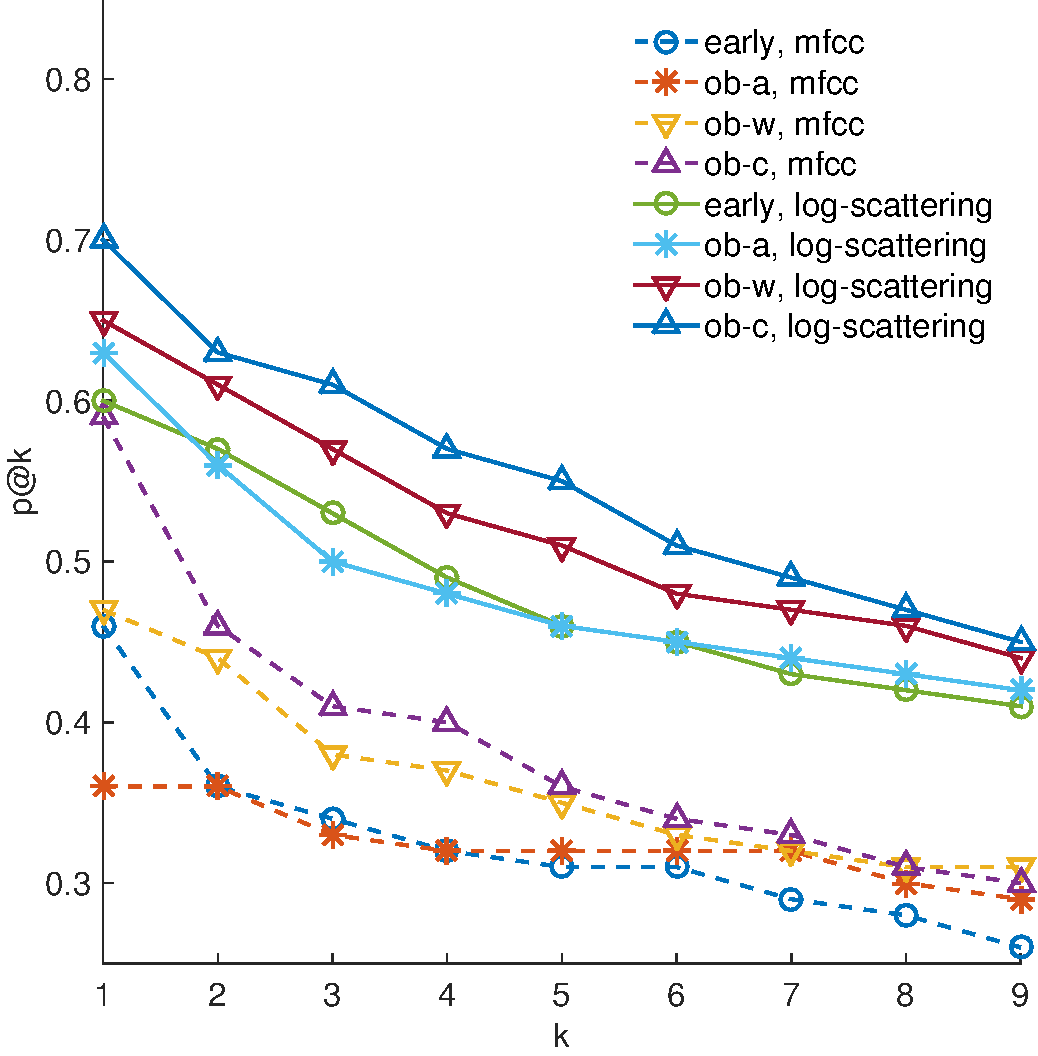
\includegraphics[width=.9\columnwidth]{gfx/ch_8/unsupervised_test2-eps-converted-to}
\caption{Acoustic scene similarity retrieval (ASSR) in the DCASE 2013 private dataset: precisions at rank $k$ ($P@k$) obtained for MFCCs and scattering with logarithmic compression, as a function of the rank $k$.}
\label{fig:ASS_1}
\end{center}
\end{figure}

\begin{figure}[t]
\begin{center}
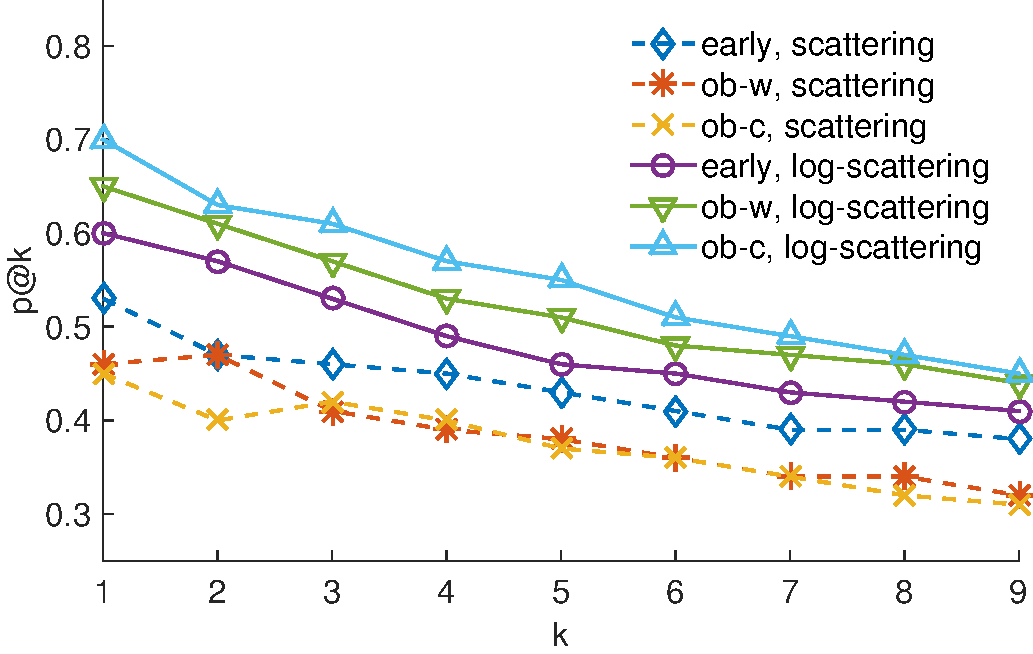
\includegraphics[width=.9\columnwidth]{gfx/ch_8/unsupervised_test1-eps-converted-to}
\caption{Acoustic scene similarity retrieval (ASSR) in the DCASE 2013 private dataset: precisions at rank $k$ ($P@k$) obtained for scattering coefficients, with and without logarithmic compression, as a function of the rank $k$.}
\label{fig:ASS_2}
\end{center}
\end{figure}

Les $P@k$ pour les différentes conditions expérimentales considérées sont affichés sur les figures~\ref{fig:ASS_1} et~\ref{fig:ASS_2}.  La figure~\ref{fig:ASS_1} illustre l'influence des approches (\emph{early} \vs~\emph{ob}) et des descripteurs  (MFCC \vs~\emph{scattering}), et la figure~\ref{fig:ASS_1} l'effet de la compression logarithmique sur les coefficients de \emph{scattering}.

\subsubsection{MFCC \vs~scattering}


Quel que soit le rang $k$ considérée, le meilleur résultat est obtenu pour les coefficients de \emph{scattering} avec une compression logarithmique en utilisant l'approche \emph{ob-c}. 

Dans l'ensemble, les coefficients \emph{log-scattering} surpassent systématiquement MFCCs. La capacité du \emph{scattering} à capturer des modulations à grande échelle améliore ainsi nettement les performances par opposition aux MFCCs qui ne décrivent qu'une enveloppe spectrale de courte durée.\\

On constate que la compression logarithmique améliore fortement les résultats pour le \emph{scattering}, en particulier pour les approches \emph{ob} qui obtiennent des résultats inférieurs à ceux de \emph{early} pour des coefficients de \emph{scattering} sans compression logarithmique (\cf~Figure~\ref{fig:ASS_2}).

\subsubsection{Approche objet \vs~early}

Pour le \emph{scattering}, les performances des deux approches \emph{ob-c} et \emph{ob-w} surpassent celles de \emph{early}, confirmant ainsi les avantages de l'utilisation d'une représentation à base d'objets pour affiner les mesures de similarité entre les scènes. 

Cependant, il convient de noter que les performances de \emph{ob-a} sont similaires à celles de \emph{early}. Ce fait tend à montrer que l'information discriminante est détruite par le moyennage des contributions de tous les centroïdes. Afin de pouvoir bénéficier d'une représentation à base d'objets, il est nécessaire de ne sélectionner que certains centroïdes représentatifs lorsqu'on les compare entre eux.

En outre, il apparaît que \emph{ob-c} est plus à même de recouvrer les similarités que \emph{ob-w}. Cette dernière observation suggère que la pondération des clusters en fonction du nombre de trames qu'ils contiennent peut se révéler être une solution limitée. En effet, rien a priori n'indique que l'information discriminante entre deux scènes ne soit contenue au sein de la majorité de leurs trames. Au contraire, ces résultats semble montrer que deux environnements de deux classes différentes peuvent partager un grand nombre de sources sonores similaires, la discrimination ne s'opérant que sur certaines.

Les mêmes observations sont faites pour les MFCCs pour un $k\leq5$. Cependant, pour un rang $k$ supérieur $5$, toutes les approches objets affichent des résultats semblables. Cela peut être dû au fait que, à un moment donné, les MFCCs ne parviennent plus à faire la distinction entre les différents événements d'une scènes, mélangeant ainsi les éléments discriminants, à ceux non informatives. Dans ce cas, l'étape de \emph{clustering} mise en œuvre dans l'approche objet et visant à regrouper les informations similaires  est rendue inutile.

\subsection{Application à la classification}

%*****************************************
%*****************************************
%*****************************************
%*****************************************
%*****************************************




